\documentclass[11pt]{article}
\usepackage[margin=2.5cm]{geometry}
\usepackage{graphicx,booktabs,hyperref,amsmath}
\usepackage[T1]{fontenc}
\hypersetup{colorlinks=true,linkcolor=black,urlcolor=blue,citecolor=black}
\title{Swapped site coordinates and a sidereal-time error in the APPLAUSE DR4 plate metadata}
\author{Qianghao Wu}
\date{November 27, 2026}
\begin{document}
\sloppy
\maketitle

\begin{abstract}
APPLAUSE Data Release~4 (DR4) is a public archive with metadata for 94{,}090 photographic plates, mostly from Hamburg, Bamberg and Potsdam. Its schema defines \texttt{site\_longitude} as the east longitude of the site, \texttt{site\_latitude} as its latitude, and \texttt{ut\_mid} as the UT of the exposure midpoint. We report two errors in these columns. (1) Four site records have the longitude and the latitude exchanged: Bamberg (18{,}681 plates), Muottas Muragl (93), Hotel Schatzalp in Davos (38) and San Miguel, Argentina (870). A test that we registered in advance shows that the exchange did not enter \texttt{ut\_mid} at Bamberg ($n=18{,}947$ timed exposures) or San Miguel ($n=858$): at the true sites, the Sun is above $-6^\circ$ at 0.13\,\% and 0.0\,\% of the midpoints, and the time shift that the exchange implies raises these fractions to 10.7\,\% and 3.5\,\%. Users who take the recorded coordinates get wrong altitudes; for example, 6.0\,\% of the archive-208 exposures then appear to be in twilight or daylight. (2) A negative control found that in the Vatican Observatory archive (archive 501, Castel Gandolfo), 40.8\,\% of the 544 DR4 midpoints have the Sun above $-6^\circ$. DR4 copies the logged time into \texttt{ut\_mid} without change. If the logged time is read as local sidereal time, 0.2\,\% of the midpoints are in daylight or twilight, and the plate centre is below $20^\circ$ altitude for 0.7\,\% of exposures, against 51.3\,\% for the DR4 midpoints. When the logged times are permuted among exposures, the same reading gives on average 41.6\,\% in daylight or twilight and 9.3\,\% below $20^\circ$. The sidereal reading changes all 543 dated midpoints (1951 May 19 to 1953 Dec 26), also those that DR4 puts at night, and leaves one of them in daylight; the median correction is 4.9\,h. We give a corrected midpoint for each exposure. The midpoints of Potsdam archives 4 and 5 are also often in daylight; we did not find the cause.
This work has not yet been reviewed by experts. The computations and the text were produced by AI models (from Anthropic and OpenAI), working under the author's direction.
\end{abstract}

\section{Introduction}
The APPLAUSE project (Archives of Photographic PLates for Astronomical USE) scanned the plate collections of Hamburg, Bamberg and Potsdam, and added scans from Tartu, Tautenburg and the Vatican Observatory~\cite{enke2024}. Data Release~4~\cite{dr4} has ``metadata for 94090 plates with a total of 139539 exposures''~\cite{dr4doc} and is open to anonymous queries through a TAP service. DR4 added two archives: Bamberg North (archive 208) and the Vatican Double Astrograph (archive 501)~\cite{dr4new}. The metadata were transcribed by hand from plate envelopes, logbooks and observer notes, which Enke et al.\ call ``a time-consuming process prone to errors''~\cite{enke2024}. The project then converted the raw times to UT and computed the heliocentric Julian date and the air mass from the times, the site and the pointing~\cite{enke2024}.

Plate times and site coordinates matter for every user who computes an altitude, an air mass or a barycentric time, and for every search for a moving object. Two recent searches used APPLAUSE plates. Graham~\cite{graham2026} used APPLAUSE DR4 Potsdam exposures in a prediscovery search for Pluto. Murtagh et al.~\cite{murtagh2026} searched DASCH and APPLAUSE plates for the distant object 2026~ED$_{138}$ and checked plate times. In the sections that we read, the only date error that they report is a $+1$\,day offset in SuperCOSMOS and STScI POSS-I dates. In the Harvard DASCH archive, an error of the opposite kind is known: the logged local mean time of J.\,H.~Metcalf's plates was read as local sidereal time~\cite{wu2026metcalf}.

We searched for an earlier report of the errors in this paper. We searched the two public collections of AI-produced research results, the archives where such results are posted, Zenodo and the web (2026 Nov 27). The only APPLAUSE result in these collections is Graham's Pluto search, and it does not report these errors. We did not find an earlier report. This search cannot exclude a report in a place that we did not search, for example an APPLAUSE help-desk note.

\section{Data}
We read the DR4 tables \texttt{applause\_dr4.plate} and \texttt{applause\_dr4.exposure} through the anonymous TAP service (\url{https://www.plate-archive.org/tap/sync}) on 2026 Nov 27. The column descriptions in \texttt{tap\_schema.columns} are:
\begin{itemize}
\item \texttt{site\_longitude}: ``East longitude of the observing site, in decimal degrees'';
\item \texttt{site\_latitude}: ``Latitude of the observing site, in decimal degrees'';
\item \texttt{ut\_mid}: ``UT date and time at the mid-point of sub-exposure''.
\end{itemize}
A \emph{timed exposure} has \texttt{jd\_mid}, a non-empty \texttt{time\_orig\_start} (the logged start time), and an exposure time above zero. A \emph{block} is one archive at one site with at least 50 timed exposures. There are 26 blocks.

For each midpoint we compute the altitude $h$ of the Sun at the site, with the low-precision solar formulae of Meeus (error below $0.02^\circ$) and no refraction. The verification stage repeated the main values with the solar position of astropy. $D_6$ is the fraction of midpoints with $h>-6^\circ$ (the Sun above the limit of civil twilight). $D_0$ is the fraction with $h>0^\circ$. $M$ is the circular mean of the local apparent solar time, minus 24\,h; a programme of night exposures centred on midnight has $M\approx0$. The placebo value of $D_6$ is the mean over 200 sets of midpoints, each moved by a random shift between $-12$ and $+12$\,h. Table~\ref{tab:blocks} gives these numbers for all blocks.

\begin{table}[t]
\centering\small
\begin{tabular}{rlrrrrr}\toprule
Archive & Site & $n$ & $D_6$ (\%) & $D_0$ (\%) & $M$ (h) & placebo $D_6$ (\%)\\\midrule
1 & Potsdam-Telegrafenberg & 5{,}050 & 4.1 & 4.1 & $-0.63$ & 55\\
2 & Potsdam-Telegrafenberg & 979 & 0.0 & 0.0 & $-0.50$ & 59\\
4 & Potsdam-Telegrafenberg & 98 & 27.6 & 26.5 & $-1.03$ & 66\\
5 & Potsdam-Telegrafenberg & 61 & 67.2 & 62.3 & $-10.98$ & 58\\
101 & Hamburg-Bergedorf & 14{,}039 & 0.8 & 0.8 & $-1.26$ & 55\\
102 & Hamburg-Bergedorf & 6{,}501 & 7.8 & 7.5 & $-1.20$ & 55\\
103 & Hamburg-Bergedorf & 9{,}624 & 2.0 & 1.7 & $-0.98$ & 54\\
104 & Calar Alto & 3{,}194 & 0.1 & 0.1 & $+0.13$ & 54\\
105 & Bonn & 1{,}427 & 0.0 & 0.0 & $-1.43$ & 55\\
106 & Hamburg-Bergedorf & 4{,}943 & 0.1 & 0.1 & $-0.48$ & 55\\
107 & Hamburg-Bergedorf & 2{,}223 & 0.1 & 0.1 & $-1.48$ & 57\\
108 & La Silla & 1{,}251 & 0.3 & 0.3 & $+0.03$ & 56\\
109 & Hamburg-Bergedorf & 2{,}025 & 2.2 & 2.2 & $-0.79$ & 55\\
110 & Hamburg-Bergedorf & 901 & 8.0 & 4.4 & $-0.91$ & 62\\
111 & Hamburg-Bergedorf & 2{,}119 & 1.4 & 1.2 & $-0.53$ & 52\\
202 & Boyden & 2{,}718 & 0.0 & 0.0 & $-1.36$ & 54\\
203 & Boyden & 12{,}565 & 1.1 & 1.1 & $-1.71$ & 53\\
204 & Mount John & 5{,}266 & 0.2 & 0.2 & $-0.42$ & 50\\
205 & San Miguel (true site) & 858 & 0.0 & 0.0 & $-0.07$ & 54\\
206 & Boyden & 693 & 0.0 & 0.0 & $-1.65$ & 53\\
207 & Boyden & 698 & 0.0 & 0.0 & $-1.28$ & 52\\
208 & Bamberg (true site) & 18{,}947 & 0.1 & 0.1 & $-0.97$ & 56\\
208 & Muottas Muragl (true site) & 93 & 1.1 & 0.0 & $-3.25$ & 50\\
301 & Tartu & 2{,}805 & 0.1 & 0.1 & $-1.70$ & 52\\
401 & Tautenburg & 4{,}083 & 0.5 & 0.0 & $+0.66$ & 55\\
501 & Castel Gandolfo & 544 & 40.8 & 32.4 & $-2.96$ & 59\\
\bottomrule\end{tabular}
\caption{Sun altitude at the DR4 midpoints, per block. $n$: timed exposures. $D_6$, $D_0$: fraction of midpoints with the Sun above $-6^\circ$ and $0^\circ$. $M$: circular mean of the local apparent solar time minus 24\,h. Placebo: $D_6$ after random shifts of up to $\pm12$\,h. For the three swapped sites, the coordinates are exchanged back (``true site'').}
\label{tab:blocks}
\end{table}

\section{Swapped site coordinates}\label{sec:swap}
A count of plates by archive, site name and coordinates gives 31 site records. In four of them, the longitude and the latitude are exchanged (Table~\ref{tab:swap}). Bamberg is near $49.88^\circ$\,N, $10.89^\circ$\,E, but DR4 gives longitude 49.8845 and latitude 10.8881. San Miguel is near $34.56^\circ$\,S, $58.73^\circ$\,W, but DR4 gives longitude $-34.5567$ and latitude $-58.7317$. The two Davos sites have longitudes near $46.5^\circ$ and latitudes near $9.9^\circ$, which is the reverse of Davos. The four records hold 19{,}682 plates. We checked them by geography only, to about $0.01^\circ$.

Of the other named sites with coordinates, all agree with their names except one. The Bonn record (7.068\,E, 50.163\,N) is about $0.57^\circ$ south of Bonn (about $50.73^\circ$\,N). It can be the Hoher List station of the Bonn observatory (about $6.85^\circ$\,E, $50.16^\circ$\,N); this is not confirmed. Three archive-208 site records (53 plates) have no coordinates.

\begin{table}[t]
\centering\small
\begin{tabular}{llrrr}\toprule
Archive & Site name in DR4 & longitude & latitude & Plates\\\midrule
208 & Dr. Remeis-Observatory, Bamberg, Germany & 49.8845 & 10.8881 & 18{,}681\\
208 & Muottas Muragl, Switzerland & 46.5217 & 9.9025 & 93\\
208 & Hotel Schatzalp, Davos, Switzerland & 46.8014 & 9.8147 & 38\\
205 & Observatorio de Fisica Cosmica, San Miguel, Argentina & $-34.5567$ & $-58.7317$ & 870\\
\bottomrule\end{tabular}
\caption{The four DR4 site records with longitude and latitude exchanged. Columns: \texttt{site\_longitude} and \texttt{site\_latitude}.}
\label{tab:swap}
\end{table}

\subsection{Did the exchange enter the UT midpoints?}
If DR4 had converted logged local mean time to UT with the recorded longitude, the true UT would be $\texttt{ut\_mid} + (\lambda_\mathrm{rec}-\lambda_\mathrm{true})/15$\,h, that is $+2.60$\,h at Bamberg and $+1.61$\,h at San Miguel. If the logs were in zone time or UT, the exchange has no effect on \texttt{ut\_mid}. We wrote down the test before we computed any Sun altitude (\texttt{PROTOCOL.md} in this record; git commit \texttt{53538d8}, 2026 Nov 27 09:22:22 CET; the commit log is \texttt{data/GIT\_LOG.txt}). For each swapped block with at least 50 timed exposures:
\begin{itemize}
\item ``the exchange entered UT'' if $D_6\ge5\,\%$, $D_6$ after the shift is at most $D_6/3$, an exact one-sided sign test on the exposures that change between day and night gives $p<0.01$, and $|M+\Delta|<1$\,h;
\item ``the exchange did not enter UT'' if $D_6<3\,\%$ and $|M|<1$\,h at the true site;
\item ``inconclusive'' otherwise.
\end{itemize}
Controls: a known-answer injection (a shift of $+2.60$\,h added to the times of Hamburg archive 101 must raise $D_6$ to at least 5\,\% and move $M$ by more than 1.5\,h), the random-shift placebo, and all other blocks as negative controls, with the expectation $D_6<3\,\%$ and $|M|<1$\,h.

\paragraph{Results.} At Bamberg ($n=18{,}947$), $D_6$ is 0.13\,\% at the true site and $M=-0.97$\,h. After the $+2.60$\,h shift, $D_6$ is 10.7\,\%. 2{,}004 exposures move from night to daylight or twilight with the shift and 7 move the other way. At San Miguel ($n=858$), $D_6$ is 0.0\,\% and $M=-0.07$\,h; after the $+1.61$\,h shift it is 3.5\,\%. Both blocks give ``the exchange did not enter UT''. Muottas Muragl ($n=93$) gives ``inconclusive'': $D_6$ is 1.1\,\%, but $M=-3.25$\,h. Hotel Schatzalp has fewer than 50 timed exposures and was not tested. The injection was detected: $D_6$ of archive 101 rose from 0.8\,\% to 9.2\,\% and $M$ moved from $-1.26$ to $+1.34$\,h. The placebo gives $D_6$ from 50\,\% to 66\,\% in every block.

\paragraph{A deviation.} The expectation $|M|<1$\,h for the negative controls was too strict. 12 of the 23 other blocks have $|M|\ge1$\,h, with $M$ from $-1.71$ to $-1.20$\,h if archives 4, 5 and 501 are excluded. Night programmes at these sites are centred about one hour before local midnight. The Bamberg verdict used $M=-0.97$\,h, which is near this limit. The conclusion at Bamberg rests on $D_6$ and on the 2{,}004 against 7 changes, which the $M$ criterion does not affect.

\paragraph{Effect on users.} With the recorded (exchanged) coordinates, 6.0\,\% of the timed exposures of archive 208 ($n=19{,}078$) appear to have the Sun above $-6^\circ$. Any altitude, air mass or local time that a user computes from these records is wrong. We did not check whether the DR4 air-mass and heliocentric-date columns used the recorded or the true coordinates.

\section{The Vatican archive: sidereal time read as UT}\label{sec:vatican}
\subsection{Discovery}
Archive 501 holds 544 plates of the Zeiss Double Astrograph at Castel Gandolfo (DR4 site 12.6505\,E, 41.7472\,N), one exposure each. It was a negative control in the test of Section~\ref{sec:swap}. Its $D_6$ is 40.8\,\% and its $D_0$ is 32.4\,\% (Table~\ref{tab:blocks}). The targets are stars and star fields, for example ``Nassau Sequence'', ``SA~64'' and ``Auriga'', which are observed at night.

DR4 copies the logged time into \texttt{ut\_mid} without change: for all 544 exposures, the clock time of \texttt{ut\_mid} differs from the logged midpoint $o=\texttt{time\_orig\_start}+\texttt{exptime}/2$ by at most 0.4\,s. Thus DR4 read the logged value as UT.

After we saw these numbers, we tested two fixed rules. Rule $H_B$ states that $o$ is local sidereal time (LST). Under $H_B$, the true midpoint is an instant at which the LST at Castel Gandolfo equals $o$. We take the instant nearest to the DR4 midpoint (the ``nearest'' rule). Under this rule, 222 midpoints move from daylight or twilight to night, 1 moves the other way, and $D_6$ falls from 40.8\,\% to 0.2\,\% (Fig.~\ref{fig:vat}). The other rule, $H_A$, states that $o$ is local mean time and was read as sidereal time; an error of this kind is known in DASCH~\cite{wu2026metcalf}. $H_A$ gives $D_6=48.7\,\%$. This comparison is exploratory, because we chose $H_B$ after we saw the data.

\begin{figure}[t]
\centering
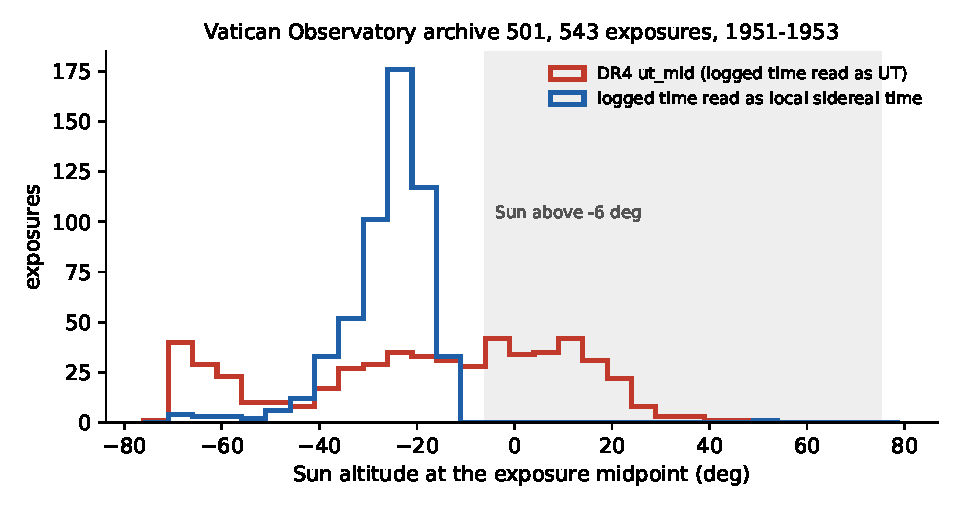
\includegraphics[width=0.8\textwidth]{fig_vatican.pdf}
\caption{Sun altitude at the midpoint of the 543 dated exposures of archive 501. Red: DR4 \texttt{ut\_mid}. Blue: the logged time read as local sidereal time (nearest instant). The grey area is $h>-6^\circ$.}
\label{fig:vat}
\end{figure}

\subsection{Tests}
\paragraph{Test registered before the computation.} Before we computed it, we registered a test with the hour angle of the plate centre (Addendum~3 of \texttt{PROTOCOL.md}). Let $\alpha$ be the recorded right ascension of the plate centre. $\mathrm{HA}_\mathrm{DR4}$ is the LST of the DR4 midpoint minus $\alpha$, and $\mathrm{HA}_B=o-\alpha$. Plates are usually taken near the meridian, so the correct reading has more exposures with $|\mathrm{HA}|<3$\,h. The rule was: $H_B$ is confirmed if the fraction with $|\mathrm{HA}_B|<3$\,h exceeds the fraction with $|\mathrm{HA}_\mathrm{DR4}|<3$\,h by at least 0.25 and an exact two-sided sign test gives $p<0.001$. The fractions are 70.2\,\% and 27.4\,\%; 241 exposures favour $H_B$ and 8 favour DR4 ($p=7\times10^{-61}$). The test passed. In the control (Hamburg archive 101, $n=13{,}785$, where DR4 already converts the logged time as sidereal time), the difference is 0.006, inside the registered limit of $\pm0.05$.

Two limits apply. First, the $p$ value does not measure the strength of the evidence for $H_B$. When we permute the logged times among the exposures, $|o-\alpha|<3$\,h holds for 63.5\,\% on average (maximum 65.8\,\% in 200 permutations); the real value, 70.2\,\%, is only a little higher. The small $p$ value comes mostly from the low DR4 value, 27.4\,\%, which shows that the DR4 midpoints are wrong. Second, in the Hamburg control, the sign test is 97 against 13 ($p=5\times10^{-17}$), although the difference is small. We did not study the cause. The same rule $H_B$ moves 107 of the daylight midpoints of archive 101 to night and none the other way, so a small part of archive 101 can have the same error.
Addendum~3 replaced a placebo of Addendum~2 that was mis-specified. The Addendum~3 text and its result file are in the same git commit (\texttt{3d66c29}), so git does not prove that the text came first; the work log states this order.

\paragraph{Controls added after the result (post hoc).} The verification stage and this paper added the controls below. They were chosen after the result was known.
\begin{itemize}
\item \emph{Permutation of the Sun test.} We gave each exposure the logged time of a random other exposure and applied $H_B$. In 50 permutations, $D_6$ is 41.6\,\% on average (minimum 38.2\,\%). The real pairing gives 0.2\,\%. So $H_B$ puts an exposure at night only when the logged time goes with its own date.
\item \emph{Altitude of the plate centre.} With the DR4 midpoint, the plate centre is below the horizon for 28.1\,\% of the exposures and below $20^\circ$ for 51.3\,\%. With $H_B$, these values are 0.2\,\% and 0.7\,\%. With permuted logged times, the fraction below $20^\circ$ is 9.3\,\% on average (minimum 7.0\,\% in 1{,}000 permutations).
\item \emph{Exposures that DR4 puts at night.} For the 322 exposures with the Sun below $-6^\circ$ at the DR4 midpoint, the plate centre is below the horizon for 23.9\,\% with the DR4 midpoint and for 0.3\,\% with $H_B$. Their median correction is 3.6\,h, and 20\,\% of them have a correction below 1\,h. These exposures have wrong midpoints too.
\end{itemize}
The verification stage computed the Sun and target altitudes independently with astropy. It got the same $D_6$ values and hour-angle counts, and target fractions within 0.6 percentage points of ours (for example 28.3\,\% against our 28.1\,\%).

\subsection{Scope and corrected midpoints}
543 of the 544 exposures are dated from 1951 May 19 to 1953 Dec 26. One record (exposure 139402, plate 96272) has the logged date 1999-12-31, a logged exposure from 23:37:30 to 00:22:30, \texttt{ut\_mid} 2000-01-01 00:00:00, and RA and Dec zero. These are placeholder values. The archive paper gives 1951--1999 for this archive~\cite{enke2024}; the end year comes from this record.

The sidereal reading changes all 543 dated midpoints, not only the 222 that DR4 puts in daylight. It leaves one of them (exposure 139045, below) in daylight. The median absolute correction is 4.9\,h and the maximum is 11.8\,h; 98.2\,\% of the corrections exceed 10\,min. The file \texttt{data/vatican\_corrected.csv} gives, for each of the 544 records, the DR4 midpoint and the corrected midpoint.

A corrected midpoint has an ambiguity of one sidereal day (23.93\,h), because the log gives the LST and a date, and the date convention is not known. The nearest rule takes the instant nearest to the DR4 midpoint. A second rule takes the instant on the logged date as a UT date. The two rules differ by one sidereal day for 222 of the 544 records. Both give $D_6=0.2\,\%$. The file gives both. No result in this paper depends on the choice.

One dated exposure is not explained by $H_B$: exposure 139045 (plate 95915, 1951 May 19, logged start 00:58, midpoint 01:02) is at Sun altitude $+50^\circ$ under the nearest rule. In May, LST 01:02 at Castel Gandolfo occurs only in daylight.

\section{Other archives}
Potsdam archives 4 and 5 (98 and 61 timed exposures, mostly 1950s and 1960s) have $D_6$ of 27.6\,\% and 67.2\,\%. Their logs are marked ``ST'', and DR4 already converts them as sidereal time. Neither $H_B$ nor $H_A$ lowers $D_6$ for them. Hamburg archives 102 and 110 have $D_6$ of 7.8\,\% and 8.0\,\%. We did not find the cause of these values; they can be errors, or daytime work such as tests. We did not examine them further.

\section{How the results were checked}
\begin{itemize}
\item \texttt{checks/rerun.py} downloads the DR4 tables (about 90\,MB) and reproduces every number in this paper. It compares 70 values and the file of corrected midpoints with \texttt{data/expected.json} and the committed file. A rerun with a fresh download in the verification stage matched all values of that stage.
\item The verification stage wrote independent code with astropy~8.0.3 for the Sun position and the VOTable parser, and with no code from the analysis. It got the same values for the swap test (Bamberg, San Miguel, injection) and for the Vatican $D_6$, $D_0$, $H_B$ and hour-angle numbers.
\item The verification stage compared the three column descriptions with a fresh query of \texttt{tap\_schema.columns}. They agree word for word.
\item The registered protocol is in git commit \texttt{53538d8} (09:22:22 CET). The first results file is in commit \texttt{1b7f1f7} (09:24:02 CET). The protocol header gave the time as ``\textasciitilde09:25''; the commit time is the evidence.
\end{itemize}

\section{Limits}
\begin{itemize}
\item We did not see the Vatican logbooks. DR4 has no logbook scans for archive 501. That the logbooks state sidereal time is our inference from the tests above; it is not confirmed. A scan of the logbooks or the APPLAUSE plate notes can confirm it.
\item The sidereal reading explains 542 of the 543 dated Vatican midpoints with respect to daylight. The hour-angle test alone is weak against a permutation (Section~\ref{sec:vatican}).
\item The true coordinates of the four swapped sites are known to us only to about $0.01^\circ$.
\item The Sun model has no refraction. Refraction matters only near the horizon and does not change the test at $h=-6^\circ$.
\item We did not check the DR4 air mass, heliocentric Julian date or the FITS headers of the scans, which DR4 computes from the same metadata.
\item The novelty claim rests on the searches listed in the introduction.
\end{itemize}

\section*{Acknowledgements}
This work has made use of data from APPLAUSE Data Release~4. Funding for APPLAUSE has been provided by DFG (German Research Foundation, Grant), Leibniz Institute for Astrophysics Potsdam (AIP), Dr. Remeis Sternwarte Bamberg (University Nuernberg/Erlangen), the Hamburger Sternwarte (University of Hamburg) and Tartu Observatory. Plate material also has been made available from Th\"uringer Landessternwarte Tautenburg, and from the archives of the Vatican Observatory.

\begin{thebibliography}{9}
\bibitem{dr4} APPLAUSE Data Release 4, Leibniz Institute for Astrophysics Potsdam, \url{https://www.plate-archive.org}, doi:\href{https://doi.org/10.17876/plate/dr.4}{10.17876/plate/dr.4}. CC0~1.0. Accessed 2026 Nov 27.
\bibitem{dr4doc} APPLAUSE, ``DR4 documentation'', \url{https://www.plate-archive.org/cms/documentation/dr4/}. Accessed 2026 Nov 27.
\bibitem{dr4new} APPLAUSE, ``What's new in DR4'', \url{https://www.plate-archive.org/cms/documentation/dr4/whats-new-in-dr4/}. Accessed 2026 Nov 27.
\bibitem{enke2024} H.~Enke, T.~Tuvikene, D.~Groote, H.~Edelmann, U.~Heber, ``Archives of Photographic PLates for Astronomical USE (APPLAUSE): Digitisation of astronomical plates and their integration into the International Virtual Observatory'', A\&A 687, A165 (2024), doi:\href{https://doi.org/10.1051/0004-6361/202348793}{10.1051/0004-6361/202348793}, arXiv:\href{https://arxiv.org/abs/2404.17355}{2404.17355}.
\bibitem{graham2026} P.~Graham, ``Candidate images of Pluto on archival plates from 1908 and 1909'' (2026), \url{https://github.com/6/clank-lab/tree/main/results/pluto-prediscovery}, doi:\href{https://doi.org/10.5281/zenodo.24387450}{10.5281/zenodo.24387450}.
\bibitem{murtagh2026} J.~Murtagh, C.~O.~Chandler, M.~Juri\'c, et al., ``A Century-Long Archival Search and Analysis of the Rubin Observatory-Discovered Dwarf Planet Candidate 2026 ED$_{138}$'', arXiv:\href{https://arxiv.org/abs/2611.02371}{2611.02371} (2026).
\bibitem{wu2026metcalf} Q.~Wu, ``A systematic time error in the DASCH metadata of J.\,H.~Metcalf's early `ma' plates, and Pluto on four Harvard plates of 1908 and 1909'' (2026), doi:\href{https://doi.org/10.5281/zenodo.24523190}{10.5281/zenodo.24523190}.
\end{thebibliography}
\end{document}
